
\documentclass[a4paper]{article}

\usepackage{INTERSPEECH_v2}

\title{Predicting age using synchronized MEG and speech recordings of children}
\name{Author Name$^1$, Co-author Name$^2$}
\address{
  $^1$Author Affiliation, Sweden\\
  $^2$Co-author Affiliation, Australia}
\email{author@university.edu, coauthor@company.com}

\usepackage{soul,color}
\newcommand{\FR}[1]{{\small \textcolor{red}{\hl{#1}}}}

\begin{document}

\maketitle
% 
\begin{abstract}
% FR: 
Evidence suggests that there is a correlation between the synchronization of different brain areas and the development of language in children. In order to explore this correlation, we attempt to predict the age of children (4-18 years old) using synchronized magneto-encephalographic (MEG) and audio recordings of verb generation and syllable production tasks. We extract time-windowed features from both MEG and audio recordings to capture time and frequency domain signal characteristics, then investigate the correlations between audio and brain recording features. We also use regularized linear regression to predict the age of subjects using audio, MEG and MEG+audio feature sets, and obtain consistent RMSE. 
\end{abstract}


\noindent\textbf{Index Terms}: Brain Computer Interfaces, BCI, Speech Production

\section{Introduction}

The synchronization of neural oscillations between distributed brain regions has been an effective mechanistic explanation for various cognitive and perceptual processes \cite{Fries2015,Nakasaki1989,NeuralSync}. \FR{Yes -- 1 more sentence about brain synchronization and processing. A broad definition.}. For example, Doesburg {\em et al.} \cite{Doesburg2016} observed an increased synchrony during verb-generation (VG) tasks in children and adolescents \FR{relative to adults?}, and observed a significant increase in the number of synchronous regions with older adolescents, compared with younger children. Furthermore, Yu {\em et al.} \cite{Yu2014} noticed distinct profiles of de-synchrony in VG tasks for children within five age ranges (i.e., 4-6, 7-9, 10-12, 13-15, and 16-18 years of age). These findings indicate the possibility of inferring a child's age from observed MEG data, provided the ability to convey synchronicity and coordinated activity. The extraction of common spectral features such as the fast Fourier transform (FFT) magnitude and features like signal energy have shown some success with various classifiers in accurately differentiating different persons from electroencephalographic (EEG) experiments \cite{Nguyen2012} \cite{Poulos2001}. Something on MEG vs. EEG?

MEG tends to be more accurate and more appropriate vs. EEG?

We hypothesized that the accuracy of a regression model trained using a combined dataset of MEG and audio features would be greater than that of models trained with only audio and MEG respectively. Furthermore this would likely be due to the fact that the MEG data would represent the synchronicity and 

\section{Methods}

%Overview of experiments, data processing and analysis performed

\subsection{Experiments}

The experiments performed consisted of four tests conducted for work on age and sex related developmental language differences {Pang...}. Two consisted of children repeatedly producing vocalizations when prompted..., a test where subjects kept there mouths open and did not vocalize... and finally a verb generation task where... The subjects were prompted to produce a response  times for each experiment.

\subsection{Subjects}

There were 70 (36 boys and 34 girls) healthy native English speaking children who performed the experiment. Their ages ranged from 4.1-18.4 years of age. (The children's speech was also verified to show no signs of articulartory difficulties through observation?).

\begin{itemize}
\item How much more tie in to Pang papers?
\item Additional information about handedness and intelligence measures? Relating to Broca's area typically in dominant hemisphere?
\end{itemize}

\subsection{Data Collection and Preparation}

Participants were tested in a magnetically shielded room in the Neuromagnetic Lab at the Hospital for Sick Children, using a CTF 151-channel whole-head MEG system (MEG International Services Ltd., Coquitlam, BC, Canada). The system recorded the 151 MEG channels and a single audio channel with a sampling rate of 4kHz. The MEG signals were resampled at 200Hz, and band pass filtered between 0.5Hz and 100 Hz.

Muscular artifacts, and in particular ocular artifacts are a significant source of MEG signal contamination. Simple rejections of epoched data would result in nontrivial loss of collected information. Removal of electro-ocular (EOG) artifacts was therefore performed using automated Blind Source Separation (BSS) method and examining signal complexities measured by fractal dimensions. Auto-BSS filters EOG artifacts using the SOBI algorithm in AAR's implemention.

Independent component analysis (ICA) (explain a little bit, or just reference here?) was then used to determine statistically independent sub-components of the MEG recordings across all subjects. This was done by appending MEG recordings for all subjects into a single 151 channel matrix for each of the 4 tests performed using the EEGLAB toolbox \cite{Delorme04eeglab} for MATLAB.

The weight matrix produced by the ICA for each test condition was applied to each subject's recordings per respective test and the recordings (both MEG and audio separately) were separated into epochs that correspond to -500ms to +1500ms windows around each prompt a subject received to perform a test.

Features were then extracted from all epochs using openSMILE \cite{Eyben13-RDI}. 

\begin{itemize}
\item 50ms windows with 25ms overlap  
\item Number of features for each data mode
\item General feature categories, ie. statistical moments: mean, deviation, kurtosis..., FFT mag, energy,
  LPC, jitter, shimmer...
\item Why did we choose these features? Are we saying kitchen sink approach?
\end{itemize}

\subsection{Analysis Performed}

The analysis that was performed fell into two categories, in the first: features extracted were checked for correlations in an attempt to demonstrate evidence for predictive possibility, in the second: regularized linear regression models were learned to predict a subject's age.

\subsubsection{Correlation}

We used standard Pearson correlation to determine correlation between MEG and Audio features for each of our test conditions. Correlations were analyzed by plotting a map of correlation coefficients with $p < 0.01$. Additionally we also compared correlation between a combination of both feature sets and subject age.

\subsubsection{Linear Regression}

Three linear regression models to predict age were trained using the \textit{Audio}, \textit{MEG} and \textit{Audio+MEG (Fusion)} datasets respectively. Ten-fold cross-validation was used, such that each dataset was divided into 10 approximately equal groups, and each group had an approximately equivalent and nearly uniform distribution of points from each subject. A held out test set was used to report performance. Bayesian parameter optimization (using Hyperopt \cite{Bergstra2013}) of the first fold was used to determine an appropriate learning rate and regularization factor.

Would we put a regression formula here?

\section{Results}

\subsection{Components}

Plotting the dominant components derived from the ICA, we notice that for VG, PA and PDK measurements the components strongly select for activity localized around sensors located in the center-left of the frontal area. !! Placeholder, might not be using this anymore... 

\begin{figure}[t]
  \centering
  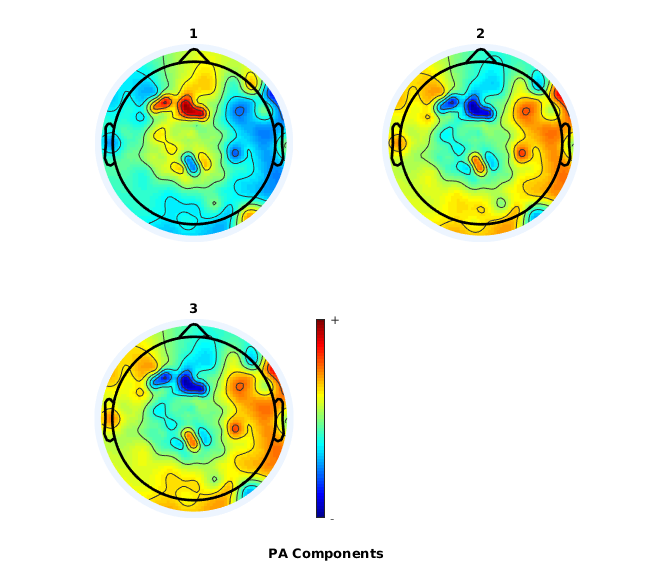
\includegraphics[width=\linewidth]{PA_components.png}
  \caption{Component weights for PDK condition, plotted over a scalp map using \cite{Delorme04eeglab}. Note that ICA may have signs flipped.}
  \label{fig:components} 
\end{figure}

\subsection{Correlations} 

\subsubsection{MEG vs. Audio Features}

We compare the correlations 

\begin{itemize}
\item Could use the correlation figures I have been generating.
\end{itemize}


\subsubsection{All Features vs. Age}

ShDo we want to just list the most correlated features here?

\subsection{Regression}

Here, talk about weights of the linear regression model, see features X,Y,Z for times t1... are the largest weights...

\begin{table}[t]
  \caption{Root mean squared error (RMSE) in years, of ten-fold cross validation for Audio, MEG, and Fusion datasets.}
  \label{tab:xvalreg}
  \centering
  \begin{tabular}{ r@{}l  r }
    \toprule
    \multicolumn{1}{c}{\textbf{Dataset}} & \multicolumn{1}{c}{\textbf{Mean}} & \multicolumn{1}{c}{\textbf{Deviation}} \\
    \midrule
    Audio~~~                        & $3.129$         &     $0.561$   \\
    MEG~~~                          & NaN             &      NaN      \\
    Fusion~~~                       & Nan             &      NaN      \\
    \bottomrule
  \end{tabular}
\end{table}

\section{Discussion}

Could say something about potential difficulty of relying on synchronicity due to the fact that correlated firing does not imply as much as once thought \cite{Moreno-Bote2014}. 

\subsection{Significance}

Frank wants to write section outlining caveats

\section{Conclusions}

Lorem Ipsum

\section{Acknowledgements}

Lorem Ipsum


\bibliographystyle{IEEEtran/bibtex/IEEEtran}

\bibliography{IS2017}


\end{document}
